\chapter{ОБЗОР} \label{chapt2}
В данной работе анализ рассматривается в контексте задачи классификации. Рассмотрим наиболее популярные на момент публикации данной работы методы анализа образов.

\section{Теория распознавания образа}

Теория распознавания образа --- раздел информатики и смежных дисциплин, развивающий основы и методы классификации и идентификации предметов, явлений, процессов, сигналов, ситуаций и т. п. объектов, которые характеризуются конечным набором некоторых свойств и признаков. Такие задачи решаются довольно часто, например, при переходе или проезде улицы по сигналам светофора. Распознавание цвета загоревшейся лампы светофора и знание правил дорожного движения позволяет принять правильное решение о том, можно или нельзя переходить улицу.

Необходимость в таком распознавании возникает в самых разных областях --- от военного дела и систем безопасности до оцифровки аналоговых сигналов.

Проблема распознавания образа приобрела выдающееся значение в условиях информационных перегрузок, когда человек не справляется с линейно-последовательным пониманием поступающих к нему сообщений и в результате его голова переключается на режим одновременности восприятия и мышления, которому такое распознавание свойственно.

Неслучайно, таким образом, проблема распознавания образа оказалась в поле междисциплинарных исследований --- в том числе в связи с работой по созданию искусственного интеллекта, а создание технических систем распознавания образа привлекает к себе всё большее внимание.

Распознавание образов --- это отнесение исходных данных к определённому классу с помощью выделения существенных признаков, характеризующих эти данные, из общей массы несущественных данных.

Классическая постановка задачи распознавания образов: близка к постановке задачи классификации и предполагает наличие некоторого базового набора заранее известных классов (набор может расширятся), и образа (не обязательно визуального) которые надо классифицировать.

Наиболее часто в задачах распознавания визуальных образов рассматриваются монохромные изображения, что даёт возможность рассматривать изображение как функцию на плоскости.

Множество же всех возможных функций $f(x, y)$ на плоскости $T$ --- есть модель множества всех изображений X. Вводя понятие сходства между образами можно поставить задачу распознавания. Конкретный вид такой постановки сильно зависит от последующих этапов при распознавании в соответствии с тем или иным подходом.

\section{Распознавание текста}
Оптическое распознавание текста является исследуемой проблемой в областях распознавания образов, искусственного интеллекта и компьютерного зрения.

Системы оптического распознавания текста требуют калибровки для работы с конкретным шрифтом; в ранних версиях для программирования было необходимо изображение каждого символа, программа одновременно могла работать только с одним шрифтом. В настоящее время больше всего распространены так называемые «интеллектуальные» системы, с высокой степенью точности распознающие большинство шрифтов. Некоторые системы оптического распознавания текста способны восстанавливать исходное форматирование текста, включая изображения, колонки и другие нетекстовые компоненты.

Точное распознавание латинских символов в печатном тексте в настоящее время возможно только если доступны чёткие изображения, такие как сканированные печатные документы. Точность при такой постановке задачи превышает 99 \%, абсолютная точность может быть достигнута только путем последующего редактирования человеком. Проблемы распознавания рукописного «печатного» и стандартного рукописного текста, а также печатных текстов других форматов (особенно с очень большим числом символов) в настоящее время являются предметом активных исследований.

Точность работы методов может быть измерена несколькими способами и поэтому может сильно варьироваться. К примеру, если встречается специализированное слово, не используемое для соответствующего программного обеспечения, при поиске несуществующих слов, ошибка может увеличиться.

Распознавание символов он-лайн иногда путают с оптическим распознаванием символов. Последний --- это оффлайн метод, работающий со статической формой представления текста, в то время как он-лайн распознавание символов учитывает движения во время письма. Например, в он-лайн распознавании, использующем PenPoint OS или планшетный ПК, можно определить, с какой стороны пишется строка: справа налево или слева направо.

Он-лайн системы для распознавания рукописного текста «на лету» в последнее время стали широко известны в качестве коммерческих продуктов. Алгоритмы таких устройств используют тот факт, что порядок, скорость и направление отдельных участков линий ввода известны. Кроме того, пользователь научится использовать только конкретные формы письма. Эти методы не могут быть использованы в программном обеспечении, которое использует сканированные бумажные документы, поэтому проблема распознавания рукописного «печатного» текста по-прежнему остается открытой. На изображениях с рукописным «печатным» текстом без артефактов может быть достигнута точность в 80~\%--90~\%, но с такой точностью изображение будет преобразовано с десятками ошибок на странице. Такая технология может быть полезна лишь в очень ограниченном числе приложений.

Ещё одной широко исследуемой проблемой является распознавание рукописного текста. На данный момент достигнутая точность даже ниже, чем для рукописного «печатного» текста. Более высокие показатели могут быть достигнуты только с использованием контекстной и грамматической информации. Например, в процессе распознания искать целые слова в словаре легче, чем пытаться проанализировать отдельные символы из текста. Знание грамматики языка может также помочь определить, является ли слово глаголом или существительным. Формы отдельных рукописных символов иногда могут не содержать достаточно информации, чтобы точно (более 98~\%) распознать весь рукописный текст.

Для решения более сложных проблем в сфере распознавания используются как правило интеллектуальные системы распознавания, такие как искусственные нейронные сети.

\section{Распознавание рукописного текста}

Распознавание рукописного ввода --- это способность компьютера получать и интерпретировать рукописный ввод. Распознавание текста может производиться «оффлайновым» методом из уже написанного на бумаге текста или «онлайновым» методом считыванием движений кончика ручки, к примеру по поверхности планшета.

Эти задачи реализованы такими разработчиками, как Paragon Software group
(система Pen Reader), iRex Technologies (система MyScript Notes), ABBYY (система
Fine Reader). У каждого из выпущенного ими продукта своя область применения.
Например, приложение «Pen Reader» работает только с динамическим вводом
рукописного текста, приложение «MyScript Notes» хоть и является более
функциональным решением в области распознавания рукописного текста, чем
предыдущее, но напротив не распознает текст в режиме реального времени, а лишь
конвертирует ранее введенный текст.

Качество распознавания оценивается как вероятность (т.е. частота) ошибки
классификации на другом конечном множестве объектов с заранее известными
ответами (тестовом множестве). Типичная система оценки каллиграфии включает извлечение признаков, распознавание объекта, принятие решения.

Достаточно полный обзор методов распознавания рукописного текста (да и текста в целом) представлен в \cite{demin}. Ниже представлены некоторые выдержки из этого обзора.
В целом сами алгоритмы распознавания можно разбить на следующие группы:

\subsection{Шаблонные методы}

Шаблонные методы преобразуют изображение отдельного символа в растровое
представление, сравнивают его со всеми шаблонами, имеющимися в базе и выбирают
шаблон с наименьшим количеством точек, отличных от входного изображения.

\subsection{Структурные методы}

Структурные методы \cite{fuk, gorlov} представляют объект как граф, узлами которого
являются элементы входного объекта, а дугами -- пространственные отношения между
ними. Методы, реализующие подобный подход, обычно работают с векторными
изображениями. Структурными элементами являются составляющие символ линии.
Так, для буквы Ф -- это вертикальный отрезок и дуга \ref{img_skelet}. Распознаваемый символ
подвергается процедуре скелетизации (утоньшению). Каждый полученный
контур скелетного представления описывается в виде последовательного набора
особых точек и «цепного» кода, состоящего из точки привязки, числа кодов и массива
направлений из текущей точки к следующей \cite{ocrai}.

\begin{figure}[h]
\centering
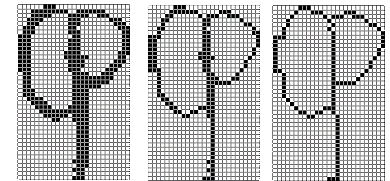
\includegraphics[width=0.75\linewidth,keepaspectratio]{images/intro_skelet_1}
\caption{Скелетизация}
\label{img_skelet}
\end{figure}

Для каждой особой точки скелетного образа вычисляются следующие признаки:
\begin{itemize}
\item нормированные координаты особой точки;
\item длина ребра до следующей вершины;
\item нормированное направление из данной точки в следующую;
\item нормированное направление входа в точку и выхода из точки;
\item кривизна дуги, соединяющая особую точку со следующей вершиной.
\end{itemize}

На рисунке \ref{img_skelet_2} условно показаны некоторые из топологических признаков. Граф
имеет пять особых точек -- $a_0$, $a_1$, $a_2$, $a_3$, $a_4$ . При обходе графа по маршруту $a_0-a_1-a_2-...$ в вершине $a_1$ условно показаны следующие признаки: вектор $R_1$ -- направление входа в точку, вектор $R_2$ -- направление выхода из точки, вектор $R_3$ -- глобальное направление
на следующую особую точку. Двунаправленный вектор $h$ показывает величину
«левого» отклонения дуги ($a_1$, $a_2$) от прямой; «правое» отклонение равно нулю.
Как видно из приведенного описания, число признаков равняется
восьмикратному числу вершин. Оно различается для разных топологических кодов, и
признаки с одинаковым номером для разных топологических кодов могут иметь
разный смысл.

\begin{figure}[h]
\centering
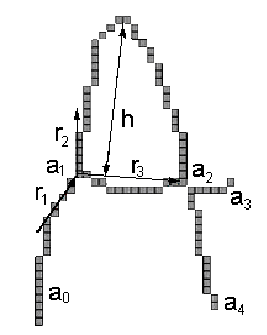
\includegraphics[width=0.25\linewidth,keepaspectratio]{images/intro_skelet_2}
\caption{Топологии скелета}
\label{img_skelet_2}
\end{figure}

Обучение метода состоит в построении деревьев распознавания для каждого из
определенных заранее (вручную или автоматически) топологических кодов.

\subsection{Признаковые методы}

Признаковые методы базируются на том, что изображению ставится в
соответствие N-мерный вектор признаков. Распознавание заключается в сравнении его
с набором эталонных векторов той же размерности. Задача распознавания, принятия
решения о принадлежности образа тому или иному классу, на основании анализа
вычисленных признаков, имеет целый ряд строгих математических решений в рамках
детерминистического и вероятностного подходов \cite{abramov, duda}. В системах распознавания
символов чаще всего используется классификация, основанная на подсчете евклидова
расстояния между вектором признаков распознаваемого символа и векторами
признаков эталонного описания. Тип и количество признаков в немалой степени
определяют качество распознавания. Формирование вектора производится во время
анализа предварительно подготовленного изображения. Данный процесс называют
извлечением признаков. Эталон для каждого класса получают путем аналогичной
обработки символов обучающей выборки.

Основные достоинства признаковых методов -- простота реализации, хорошая
обобщающая способность, хорошая устойчивость к изменениям формы символов,
низкое число отказов от распознавания, высокое быстродействие. Наиболее серьезный
недостаток этих методов -- неустойчивость к различным дефектам изображения. Кроме
того, признаковые методы обладают другим серьезным недостатком -- на этапе
извлечения признаков происходит необратимая потеря части информации о символе.
Извлечение признаков ведется независимо, поэтому информация о взаимном
расположении элементов символа утрачивается.

\subsection{Выводы}

Как видно из приведенного обзора, для всех трех методов свойственна
неполнота и ограниченность условий применения. Каждый из описанных методов сам
по себе имеет специализированную область применения: шаблонные методы
эффективнее использовать для распознавания печатных шрифтов, структурные -
рукописных при оффлайн-распознавании, признаковые---рукописных при онлайн-
распознавании.

Шаблонные, признаковые и структурные методы распознавания имеют как свои
преимущества, так и недостатки. Сравнительный анализ этих методов приведен в
таблице \ref{intro_table_review}.
\begin{table}[]
\caption{Сравнение методов распознавания}
\label{intro_table_review}
\fontsize{12pt}{14pt}\selectfont
\begin{tabularx}{\linewidth}{|l |X| X|}
\hhline{|---|}
\textbf{Методы}      & \textbf{Достоинства} & \textbf{Недостатки} \\
\hhline{|---|}
ШАБЛОННЫЕ   &   \begin{itemize}[leftmargin=*,nosep]
 \item высокая скорость распознавания;
 \item простая реализация;
 \item высокая точность распознавания дефектных символов.
\end{itemize} 

& \begin{itemize}[leftmargin=*,nosep]
\item необходимость настройки системы на
типы и размеры шрифтов;
\item не может использоваться для описания
объектов с высокой степенью изменчивости
\item может приниматься для распознавания
только печатных символов
\item надежно распознают только те шрифты,
шаблоны которых им "известны"
\item если распознаваемый шрифт хоть
немного отличается от эталонного,
шаблонные системы могут делать ошибки
даже при обработке качественных
изображений.
\item невозможность распознать шрифт, хоть
немного отличающийся от заложенного в
систему (размером, наклоном или
начертанием).
\end{itemize}           \\
\hhline{|---|}
СТРУКТУРНЫЕ & \begin{itemize}[leftmargin=*,nosep]
\item применяется для рукописных
шрифтов, имеющих, множество
вариантов начертания;
\item данные могут быть
представлены в графовой форме,
что обеспечивает инвариантность.
\end{itemize}            &  
\begin{itemize}[leftmargin=*,nosep]
\item высокую чувствительность к дефектам
изображения, нарушающим составляющие
элементы.
\item  для этих систем до сих пор не созданы
эффективные автоматизированные
процедуры обучения.
\item  трудность распознавания дефектных
символов и медленная работа.
\item  векторизация может добавить
дополнительные дефекты.
\item  как только вы представите «разорванную»
из-за дефектов печати букву, она уже не
подойдет под свое описание
\end{itemize}          \\
\hhline{|---|}
ПРИЗНАКОВЫЕ & \begin{itemize}[leftmargin=*,nosep]
\item простота реализации;
\item хорошая обобщающая спо-
собность;
\item хорошая устойчивость к
изменениям формы символов;
\item высокое быстродействие.
\end{itemize}            &  
\begin{itemize}[leftmargin=*,nosep]
\item неустойчивость к дефектам изображения;
\item при вычислении признаков
теряется существенная часть информации
\item трудно гарантировать, что к данному
классу удастся отнести только объекты
этого класса.
\end{itemize} \\
\hhline{|---|}
\end{tabularx}

\end{table}

В современных системах распознавания обычно используются все три типа
классификаторов, но основным является структурный. Два других служат для
ускорения и повышения качества распознавания. Комбинация различных методов
распознавания приводит к наилучшим результатам, примером может служить метод
структурно-пятенных эталонов компании ABBYY \cite{telkov}.


\section{Поисковые системы}
Процессы компьютеризации деятельности государственных учреждений, предприятий, быстрое развитие глобальной сети (Internet) привели к накоплению большого объема неструктурированной текстовой информации. Возникла потребность в программном обеспечении, реализующем эффективный поиск информации.

Все это привело к созданию полнотекстовых информационно-поисковых систем. Полнотекстовые Поисковые Системы (ПС)  строятся на основе информационно-поисковых языков дескрипторного типа. Информационно-технологическая структура полнотекстовых ИС включает:
\begin{itemize}
	\item хранилище документов; 
	\item глобальный словарь системы; 
	\item инвертированный индекс документов; 
	\item интерфейс ввода документов в систему; 
	\item механизм индексирования; 
	\item интерфейс запросов пользователя; 
	\item механизм поиска документов; 
	\item механизм извлечения найденных документов.
\end{itemize} 

Приведем краткий перечень типов наиболее широко используемых полнотекстовых ПС.

1. Справочно-информационные системы общего назначения, ориентированные на доступ пользователей к нормативно-правовым документам. К этим системам относятся «Консультант Плюс», «Гарант», «Кодекс» и др. 

2. Глобальные информационные службы (хост-системы), предоставляющие доступ удаленным пользователям к библиографической, полнотекстовой или другой информации. Крупнейшей в мире коммерческой службой, обеспечивающей доступ к юридической информации, является система LEXIS (США). 

3. Системы информационной поддержки деятельности правотворческих органов. Спецификой таких систем является необходимость хранения и поиска многих версий и редакций нормативно-правовых документов, с учетом вносимых поправок и изменений. 

4. Системы автоматизации делопроизводства судов, милиции и других правоохранительных органов.

5. Системы поиска информации в Интернете (Google, Yandex и др.).

Так же стоит отметить, что в настоящее время возможностями полнотекстового поиска обладают все наиболее популярные на сегодняшний день СУБД (SQL, MySQL, Postrgres).

Наибольший интерес для нас будет представлять система поиска информации Google, основанная на технологии BigTable, которая более подробно будет рассмотрена  в следующем разделе. 
\subsection{Big Table}
Big Table -- высокопроизводительная СУБД, построенная на основе Google File System (GFS), Chubby Lock Service и  других программных продуктах Google. В настоящий момент не распространяется и не используется за пределами Google, хотя клон Bigtable применяется в Агентстве национальной безопасности США.

Технология  Big Table  является на настоящий момент наиболее мощной реализацией идеологии табличной организации данных и именно она обеспечивает корпорации Google лидирующие позиции на рынке оказания услуг по полнотекстовому поиску информации в глобальной сети, а также в сотрудничестве на коммерческой основе с различными государственными учреждениями США.

Отметим, что индексирование записей в  СУБД  Big Table  не отличается от принятой в промышленных реляционных СУБД, если отбросить возможность масштабирования, т.е. размер индексов, и идеологически родственна представлению узлов в универсуме для изображений из раздела диссертации 2.5. Интерпретация. 

%\section{Место работы в обзоре}
%
%Данная работа представляет собой исследование на стыке разработки нового структурного метода с применением логико-эвристического подхода анализа ситуаций к задаче интерпретации изображений. Разработанная модель позволяет с высокой точностью описывать \textit{контурные} изображения, в то же время оставаясь инвариантной к масштабированию и поворотам, а используемые методы интерпретации доказывают возможность эффективного применения логико-эвристического подхода к задачам анализа изображений.


%\subsection{Big Data}
%Следующим этапом развития информационных технологий поиска информации после  Big Table эксперты считают технологии  Big Data.
%
%В качестве примеров таких техник, составляющих этот класс методов, приводятся:
%\begin{enumerate}
%\item цифровая обработка сигналов и обработка естественного языка (включая тональный анализ);
%\item машинное обучение, включая обучение с учителем и без учителя, а также использование моделей, построенных на базе статистического анализа или машинного обучения для получения комплексных прогнозов на основе базовых моделей;
%\item искусственные нейронные сети, сетевой анализ, оптимизация, в том числе генетические алгоритмы;
%\item распознавание образов;
%\item прогнозная аналитика;
%\item имитационное моделирование;
%\item пространственный анализ, т.е. класс методов, использующих топологическую, геометрическую и географическую информацию в данных;
%\item статистический анализ, в качестве примеров методов приводятся A/B-тестирование и анализ временных рядов;
%\item визуализация аналитических данных --- представление информации в виде рисунков, диаграмм, с использованием интерактивных возможностей и анимации, как для получения результатов, так и для использования в качестве исходных данных для дальнейшего анализа.
%\end{enumerate}
%
%Таким образом, результаты диссертации могут трактоваться как методы решения задач, относящихся  к проблематике технологий  Big Data.


%Существует множество методов распознавания изображений но в целом их можно разделить на две группы:
%\begin{enumerate}
%\item эвристические
%\item формальные
%\end{enumerate}
%
%\section{Одиночное изображение} \label{sect2_1}
%
%\begin{figure} [h] 
%  \center
%  
\includegraphics [scale=0.27] {latex}
%  \caption{TeX.} 
%  \label{img:latex}  
%\end{figure}
%
%%\newpage
%%============================================================================================================================
%\section{Длинное название параграфа, в котором мы узнаём как сделать две картинки с общим номером и названием} \label{sect2_2}
%
%А это две картинки под общим номером и названием:
%\begin{figure}[h]
%  \begin{minipage}[h]{0.49\linewidth}
%    \center{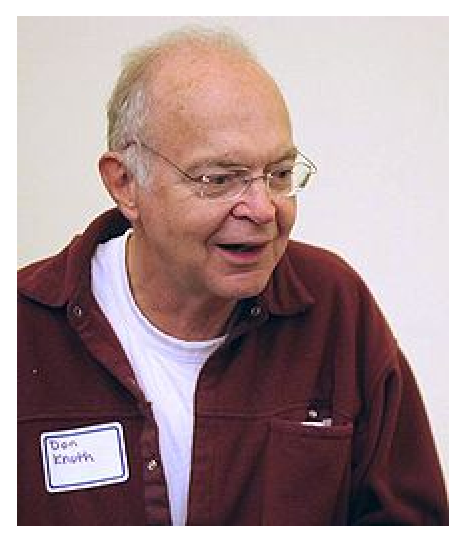
\includegraphics[width=0.5\linewidth]{knuth1} \\ а)}
%  \end{minipage}
%  \hfill
%  \begin{minipage}[h]{0.49\linewidth}
%    \center{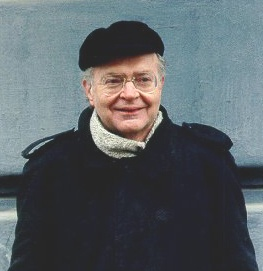
\includegraphics[width=0.5\linewidth]{knuth2} \\ б)}
%  \end{minipage}
%  \caption{Очень длинная подпись к изображению, на котором представлены две фотографии Дональда Кнута}
%  \label{img:knuth}  
%\end{figure}
%
%%\newpage
%%============================================================================================================================
%\section{Пример вёрстки списоков} \label{sect2_3}
%
%\noindent Нумерованный список:
%\begin{enumerate}
%  \item Первый пункт.
%  \item Второй пункт.
%  \item Третий пункт.
%\end{enumerate}
%
%\noindent Маркированный список:
%\begin{itemize}
%  \item Первый пункт.
%  \item Второй пункт.
%  \item Третий пункт.
%\end{itemize}
%
%\noindent Вложенные списки:
%\begin{itemize}
%  \item Имеется маркированный список.
%  \begin{enumerate}
%    \item В нём лежит нумерованный список,
%    \item в котором
%    \begin{itemize}
%      \item лежит ещё один маркированный список.
%    \end{itemize}    
%  \end{enumerate}
%\end{itemize}
%
%
%\clearpage